% !TEX root = ../main.tex
\subsection*{Languages} \label{ssec::languages}

\begin{table*}[b]%
    \begin{DndTable}[width=\linewidth]{X}
        \centering
        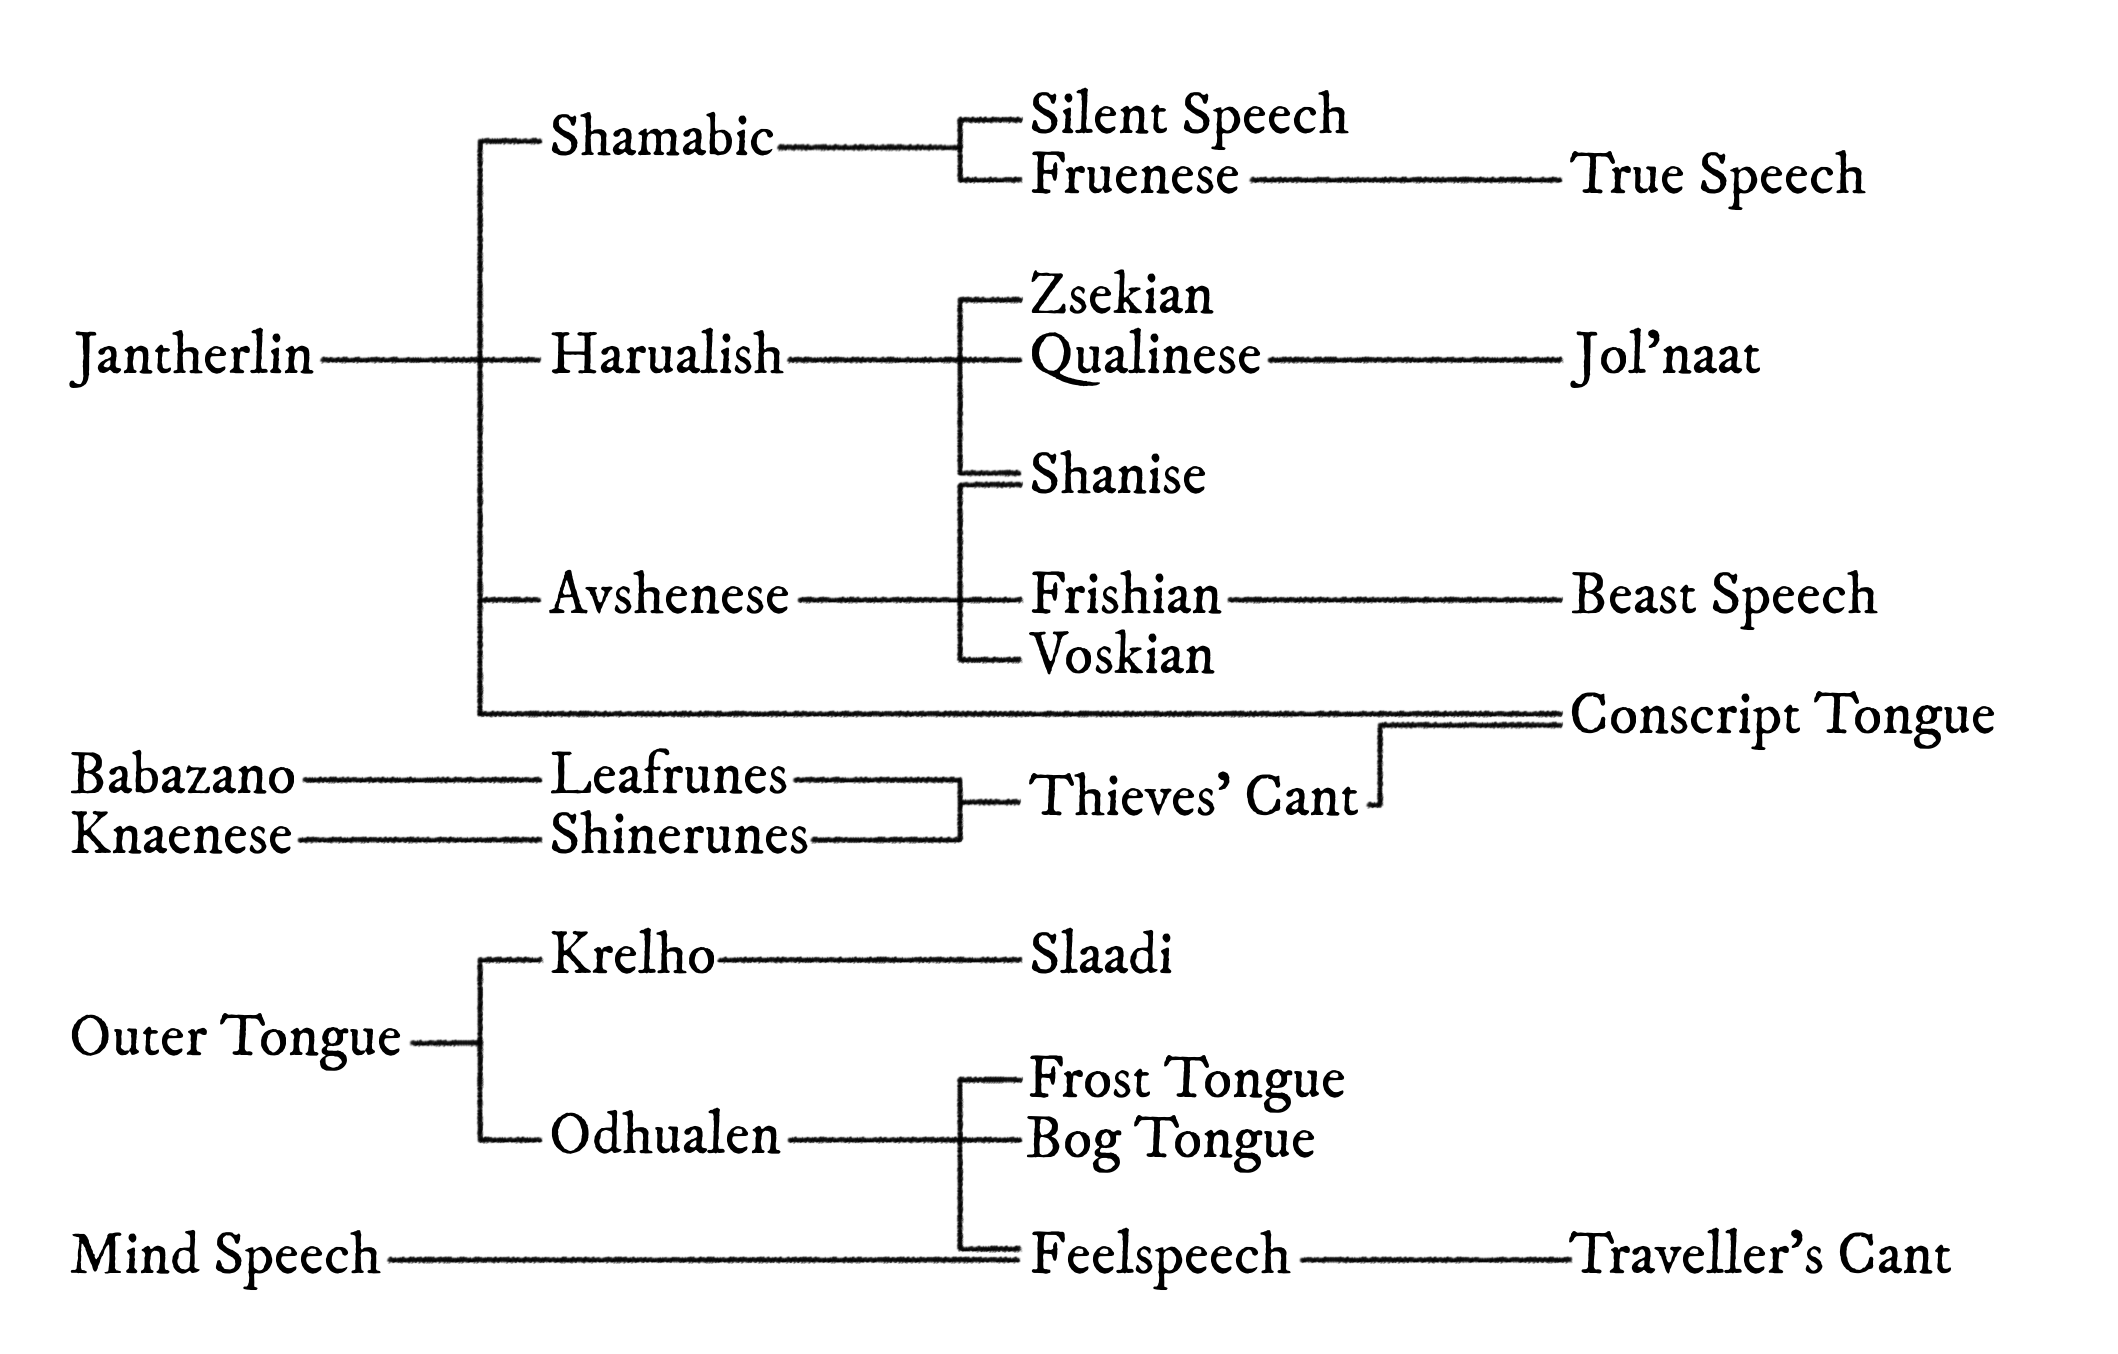
\includegraphics[width=0.99\textwidth]{01yuadrem/img/22languages_map.png}
    \end{DndTable}
\end{table*}

A great variety of languages permeate Yuadrem, both of natural spawn and artificial design.
While it is impossible to identify each tongue and its variations, many efforts have been done over the years to classify the common ones.

Based on lexical and grammatical similarities, languages are separated into four generations, and five distinct families.
The following tables classify these languages, pointing to their script and original speakers.

% As is discussed in the following pages, your country of origin determines your language more than your kin.
% Despite this, some languages are indeed associated to certain kins, as they were the original speakers.

\begin{DndTable}[width=\linewidth, header=First Generation]{p{2.6cm}p{2.6cm}X}
    \textbf{Language}  & \textbf{Original Speakers} & \textbf{Script} \\
    Jantherlin         & Ets                        & Varies \\
    Babazano           & Marsets                    & - \\
    Knaenese           & Naenks \& Tsaneks          & Knaenese \\
    Outer Tongue       & -                          & Outer Tongue \\
    Mind Speech        & Zaloths                    & -
\end{DndTable}

\begin{DndTable}[width=\linewidth, header=Second Generation]{p{2.6cm}p{2.6cm}X}
    \textbf{Language}  & \textbf{Original Speakers} & \textbf{Script} \\
    Shamabic           & Oths                       & Shamabic \\
    Harualish          & Irds                       & Harualish \\
    Avshenese          & Gats                       & Avshenese \\
    Leafrunes          & Marsets                    & Leafrunes \\
    Shinerunes         & Naenks \& Tsaneks          & Shinerunes \\
    Seedspeech         & Gannagian Tsaneks          & - \\
    Krelho             & Tortles \& Grungs          & Krelho \\
    Odhualen           & Umans                      & Outer Tongue
\end{DndTable}

\begin{DndTable}[width=\linewidth, header=Third Generation]{p{2.6cm}p{3.2cm}X}
    \textbf{Language}  & \textbf{Original Speakers} & \textbf{Script} \\
    Silent Speech      & Oths                       & - \\
    Fruenese           & Sulian Oths                & Fruenese \\
    Zsekian            & Dratl Irds                  & Harualish \\
    Qualinese          & Jenkashian Irds            & Harualish \\
    Shanise            & Northern Irds \& Gats      & Shanise \\
    Frishian           & Jorea \& Dzorvepem         & Avshenese \\
    Voskian            & Voskferm \& Voskgrit       & Avshenese \\
    Thieves' Cant      & Rogues \& Thieves          & Thieves' Cant \\
    Slaadi             & Slaads                     & Krelho \\
    Feelspeech         & Zaloths \& Umans           & -
\end{DndTable}

\begin{DndTable}[width=\linewidth, header=Fourth Generation]{p{2.6cm}p{3.2cm}p{2.2cm}}
    \textbf{Language}  & \textbf{Original Speakers} & \textbf{Script} \\
    True Speech        & Palegna \& Sulia           & - \\
    Jol'naat           & Jenkash                    & - \\
    Beast Speech       & Jorea                      & - \\
    Conscript Tongue   & Cabb Goem-Rlamesh          & - \\
    Traveler's Cant    & Zaloths \& Umans           & Traveler's Cant
\end{DndTable}

% \subsubsection{First Generation}
% \paragraph{Old Tongue} A very complicated and intricate language spoken by the tall kin, the original settlers of Yuadrem.
% It's spoken form involves various complex articulations and the definition of a word can vary greatly based on the context.
% Additionally, each tall one had their own personal version of the written form, and others would understand it as much as they understood the individual.
% % This makes the reading of the old tongue extremely difficult for the kin that remain in the world, since understanding a particular tall one's scribbles essentially requires understanding their own version of the language.
% % Nowadays, only scholars and archaeologists understand the language, and it is not normally used anywhere.
% \paragraph{Marset Tongue} Every marset is already able to speak this strange, repetitive language.
% The marset tongue only has ten consonants, and ten verbs.
% % The rest of their vocabulary is built up from there, making their language very difficult to speak or understand by kins other than the marsets.
% Marset tongue can be spoken in one of two ways: soundlessly, through lip reading, or screamed as loud as possible, with no middle ground.
% The language cannot be written down.
% \paragraph{Naenk Tongue} Short words and strong consonants define the naenk tongue.
% Lacking lips and teeth, naenks make heavy use of their alveolar ridge and hard palate to produce syllables.
% The written form of the language involves carving lines and holes onto bark or stone.
% \paragraph{Outer Tongue}
% \paragraph{Mind Speech}

% \subsubsection{Second Generation}
% \paragraph{Dust Tongue}
% \paragraph{Ird Tongue}
% \paragraph{Gat Tongue}
% \paragraph{Leafrunes} Very easy to learn, but kept secret by the archer kin.
% A marset will teach this set of runes only to creatures that it deeply trusts, and only if it's strictly necessary.
% Ten leafrunes exist, all of which are used individually and to convey very simple meaning.
% % \textit{colony}, \textit{danger}, \textit{fun place}, \textit{hiding spot}, \textit{observation point}, \textit{predators}, \textit{road}, \textit{sacred place}, \textit{source of food}, and \textit{source of materials}.
% \paragraph{Shinerunes}
% \paragraph{Krelho}
% \paragraph{Nomad Tongue}

% \subsubsection{Third Generation}
% \paragraph{Silent Speech}
% \paragraph{Standard Language}
% \paragraph{Zsek Tongue}
% \paragraph{Qul Tongue}
% \paragraph{North Tongue}
% \paragraph{Beetle Tongue}
% \paragraph{Gilded Tongue}
% \paragraph{Thieves' Cant}
% \paragraph{Slaadi}
% \paragraph{Frost Tongue}
% \paragraph{Bog Tongue}
% \paragraph{Feelspeech}

% \subsubsection{Fourth Generation}
% \paragraph{True Speech}
% \paragraph{Jol'naat}
% \paragraph{Beast Speech}
% \paragraph{Conscript Language}
% \paragraph{Traveler's Cant}
